\documentclass[]{beamer}

% Default size A0
% \usepackage[scale=1.1, size=a0]{beamerposter} % use scale from 1.1 to 1.2

% Size A1
% \usepackage[scale=0.77, size=a1]{beamerposter} % use scales around 0.8

% Use custom size to set poster's width and height.
\usepackage[scale=1.2, size=custom, width=120, height=100]{beamerposter} % use scale from 1.1 to 1.2
\usetheme{vegaposter} 


\addbibresource{refs.bib}
\usepackage{lipsum}

\title{On the broccoli fractional structure}
\author{Alexander Rosenbaum, Noname Student}
\supervisor{Group Supervisor 1, Group Supervisor 2}
\researchgroup{Important questions of stochastic calculus}

\begin{document}
\nocite{*} % This is needed to make sure that all references are included in the bibliography

\begin{frame}[t]
    \begin{columns}[t] % The whole poster consists of three major columns, the second of which is split into two columns twice - the [t] option aligns each column's content to the top
     
    \begin{column}{\lrmargin}\end{column} % Empty spacer column
    
    \begin{column}{\onecolwid} % The first column
     
    %----------------------------------------------------------------------------------------
    %	INTRODUCTION
    %----------------------------------------------------------------------------------------
    
    \begin{block}{Introduction}
    
    Lorem ipsum dolor \textbf{sit amet}, consectetur adipiscing elit. Sed commodo molestie porta. Sed ultrices scelerisque sapien ac commodo \cite{Black1976}. Donec ut volutpat elit. Sed laoreet accumsan mattis. Integer sapien tellus, auctor ac blandit eget, sollicitudin vitae lorem. Praesent dictum tempor pulvinar. Suspendisse potenti. Sed tincidunt varius ipsum, et porta nulla suscipit et. Etiam congue bibendum felis, ac dictum augue cursus a. \textbf{Donec} magna eros, iaculis sit amet placerat quis, laoreet id est. In ut orci purus, interdum ornare nibh. 
    
    \end{block}
    
    %----------------------------------------------------------------------------------------
    %	OBJECTIVES
    %----------------------------------------------------------------------------------------
    
    \begin{alertblock}{Objectives}
    
    Lorem ipsum dolor sit amet, consectetur, nunc tellus pulvinar tortor, commodo eleifend risus arcu sed odio:
    \begin{itemize}
    \item Mollis dignissim, magna augue tincidunt dolor, interdum vestibulum urna
    \item Sed aliquet luctus lectus, eget aliquet leo ullamcorper consequat. Vivamus eros sem, iaculis ut euismod non, sollicitudin vel orci.
    \item Nascetur ridiculus mus.  
    \item Euismod non erat. Nam ultricies pellentesque nunc, ultrices volutpat nisl ultrices a.
    \end{itemize}
    
    \end{alertblock}
    
    %------------------------------------------------
    \begin{block}{Problem statement}
    Pellentesque pulvinar, nibh ac malesuada accumsan, urna nunc convallis tortor, ac vehicula nulla tellus eget nulla.
    Nullam lectus tortor, \textit{consequat tempor hendrerit} quis, vestibulum in diam. Maecenas sed diam augue.
    
    This statement requires citation \cite{Heston1993}.
    Suspendisse potenti. Sed tincidunt varius ipsum, et porta nulla suscipit et. Etiam congue bibendum felis, 
    ac dictum augue cursus a.
    \end{block}
    
    %----------------------------------------------------------------------------------------
    
    \end{column} % End of the first column
    
    \begin{column}{\sepwid}\end{column} % Empty spacer column
    
    \begin{column}{\twocolwid} % Begin a column which is two columns wide (column 2)
    
    \begin{columns}[t,totalwidth=\twocolwid] % Split up the two columns wide column
    
    \begin{column}{\onecolwid}\vspace{-.6in} % The first column within column 2 (column 2.1)
    
    %----------------------------------------------------------------------------------------
    %	MATERIALS
    %----------------------------------------------------------------------------------------
    
    \begin{block}{Materials}
    
    The following materials were required to complete the research:
    
    \begin{itemize}
    \item Curabitur pellentesque dignissim
    \item Eu facilisis est tempus quis
    \item Duis porta consequat lorem
    \item Eu facilisis est tempus quis
    \end{itemize}
    
    The materials were prepared according to the steps outlined below:
    
    \begin{enumerate}
    \item Curabitur pellentesque dignissim
    \item Eu facilisis est tempus quis
    \item Duis porta consequat lorem
    \item Curabitur pellentesque dignissim
    \end{enumerate}
    
    \end{block}
    
    %----------------------------------------------------------------------------------------
    
    \end{column} % End of column 2.1
        
    \begin{column}{\onecolwid}\vspace{-.6in} % The second column within column 2 (column 2.2)
    
    %----------------------------------------------------------------------------------------
    %	METHODS
    %----------------------------------------------------------------------------------------
    
    \begin{block}{Methods}
    
    Lorem ipsum dolor \textbf{sit amet}, consectetur adipiscing elit. Sed laoreet accumsan mattis. Integer sapien tellus, auctor ac blandit eget, sollicitudin vitae lorem. Praesent dictum tempor pulvinar. Suspendisse potenti. Sed tincidunt varius ipsum, et porta nulla suscipit et. Etiam congue bibendum felis, ac dictum augue cursus a. \textbf{Donec} magna eros, iaculis sit amet placerat quis, laoreet id est. In ut orci purus, interdum ornare nibh. Pellentesque pulvinar, nibh ac malesuada accumsan, urna nunc convallis tortor, ac vehicula nulla tellus eget nulla. Nullam lectus tortor, \textit{consequat tempor hendrerit} quis, vestibulum in diam. Maecenas sed diam augue.
    
    \end{block}
    
    %----------------------------------------------------------------------------------------
    
    \end{column} % End of column 2.2
    
    \end{columns} % End of the split of column 2 - any content after this will now take up 2 columns width
    
    %----------------------------------------------------------------------------------------
    %	IMPORTANT RESULT
    %----------------------------------------------------------------------------------------
    
    \begin{alertblock}{Broccoli is rough!}
    
    Lorem ipsum dolor \textbf{sit amet}, consectetur adipiscing elit. Sed commodo molestie porta. Sed ultrices scelerisque sapien ac commodo. Donec ut volutpat elit.
    
    \end{alertblock} 
    
    %----------------------------------------------------------------------------------------
    
    \begin{columns}[t,totalwidth=\twocolwid] % Split up the two columns wide column again
    
    \begin{column}{\onecolwid} % The first column within column 2 (column 2.1)
    
    %----------------------------------------------------------------------------------------
    %	MATHEMATICAL SECTION
    %----------------------------------------------------------------------------------------
    
    \begin{block}{Mathematical Section}
    
    Nam quis odio enim, in molestie libero. Vivamus cursus mi at nulla elementum sollicitudin. Nam quis odio enim, in molestie libero. Vivamus cursus mi at nulla elementum sollicitudin.
      
    \begin{equation}
    E = mc^{2}
    \label{eqn:Einstein}
    \end{equation}
    
    Nam quis odio enim, in molestie libero. Vivamus cursus mi at nulla elementum sollicitudin. Nam quis odio enim, in molestie libero. Vivamus cursus mi at nulla elementum sollicitudin.
    
    \begin{equation}
    \cos^3 \theta =\frac{1}{4}\cos\theta+\frac{3}{4}\cos 3\theta
    \label{eq:refname}
    \end{equation}    
    \end{block}
    
     \textbf{Donec} magna eros, iaculis sit amet placerat quis, laoreet id est. In ut orci
    purus, interdum ornare nibh.
    
    %----------------------------------------------------------------------------------------
    
    \end{column} % End of column 2.1
    
    \begin{column}{\onecolwid} % The second column within column 2 (column 2.2)
    
    %----------------------------------------------------------------------------------------
    %	RESULTS
    %----------------------------------------------------------------------------------------
    
    \begin{block}{Results}
    
    \begin{figure}
    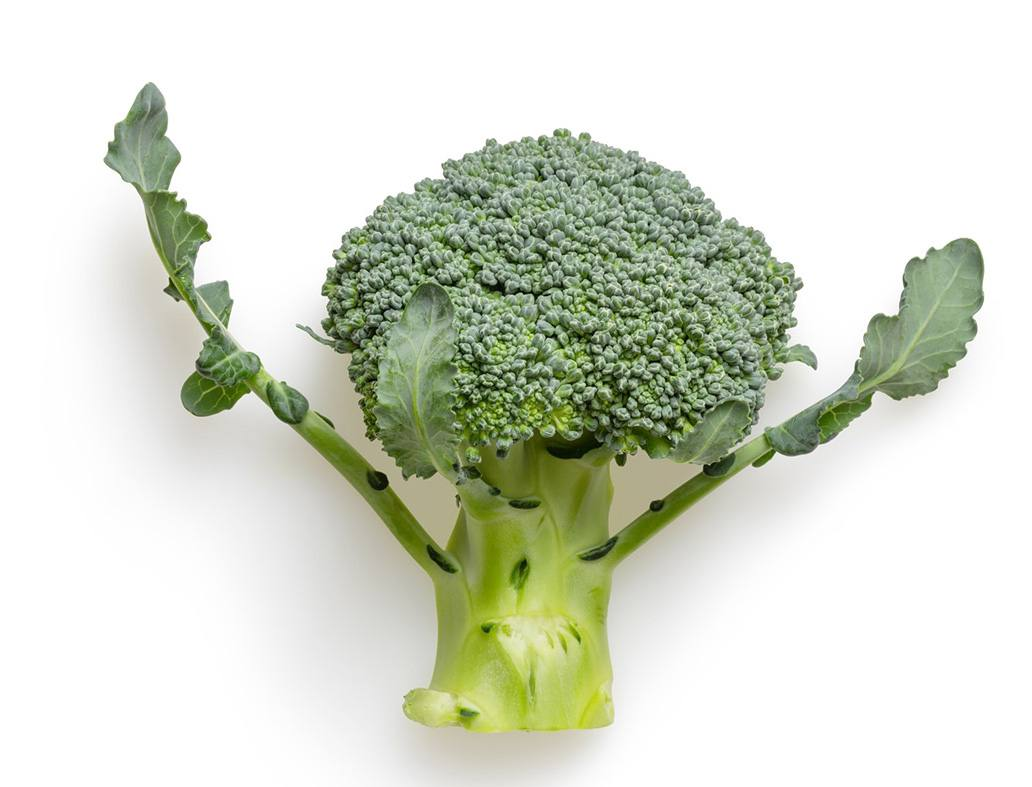
\includegraphics[width=0.8\linewidth]{figures/placeholder.jpg}
    \caption{Figure caption}
    \end{figure}
    
    Nunc tempus venenatis facilisis. Curabitur suscipit consequat eros non porttitor:
    
    \begin{table}
    \vspace{2ex}
    \begin{tabular}{l l l}
    \hline
    \textbf{Measurements} & \textbf{Dimension estimator $\hat D$} \\
    \hline
    Try 1 & 2.66 \\
    \hline
    \end{tabular}
    \caption{Empirical analysis of the Hausdorff dimension}
    \end{table}
    
    \end{block}
    
    %----------------------------------------------------------------------------------------
    
    \end{column} % End of column 2.2
    
    \end{columns} % End of the split of column 2
    
    \end{column} % End of the second column
    
    \begin{column}{\sepwid}\end{column} % Empty spacer column
    
    \begin{column}{\onecolwid} % The third column
    
    %----------------------------------------------------------------------------------------
    %	CONCLUSION
    %----------------------------------------------------------------------------------------
    
    \begin{block}{Conclusion}
    Nunc tempus venenatis facilisis. \textbf{Curabitur suscipit} consequat eros non porttitor. Sed a massa dolor, id ornare enim. Fusce quis massa dictum tortor \textbf{tincidunt mattis}. Donec quam est, lobortis quis pretium at, laoreet scelerisque lacus. Nam quis odio enim, in molestie libero. Vivamus cursus mi at \textit{nulla elementum sollicitudin}.

    Maecenas ultricies feugiat velit non mattis. Fusce tempus arcu id ligula varius dictum. 
    \begin{itemize}
    \item Curabitur pellentesque dignissim
    \item Eu facilisis est tempus quis
    \item Duis porta consequat lorem
    \end{itemize}
    
    Donec ut volutpat elit. Sed laoreet accumsan mattis. Integer sapien tellus, auctor ac blandit eget, sollicitudin vitae lorem. Praesent dictum tempor pulvinar. Suspendisse potenti. Follow us in \href{https://t.me/vega_institute}{Telegram}. Sed tincidunt varius ipsum, et porta nulla suscipit et. Etiam congue bibendum felis, ac dictum augue cursus a.
    
    \end{block}
    
    %----------------------------------------------------------------------------------------
    %	REFERENCES
    %----------------------------------------------------------------------------------------
    
    \begin{block}{References}
    
%    \nocite{*} % Insert publications even if they are not cited in the poster
    \printbibliography \vspace{0.75in}
    
    \end{block}
    
    \end{column} % End of the third column
    
    \begin{column}{\lrmargin}\end{column} % Empty spacer column
    
    \end{columns} % End of all the columns in the poster
    \end{frame} % End of the enclosing frame
\end{document}